% =====================================================================
%  GEMMA MONSTERS — team brief
%  Compile with pdfLaTeX. Run twice.
% =====================================================================
\documentclass[11pt]{article}

\usepackage[T1]{fontenc}
\usepackage[utf8]{inputenc}
\usepackage{lmodern}
\usepackage{microtype}
\usepackage[margin=0.85in,headheight=15pt,footskip=26pt]{geometry}
\usepackage{parskip}
\usepackage{enumitem}
\usepackage{booktabs}
\usepackage{tabularx}
\usepackage{array}
\usepackage[table]{xcolor}
\usepackage{tikz}
\usetikzlibrary{arrows.meta,positioning,shapes.geometric,fit,calc}
\usepackage[most]{tcolorbox}
\usepackage{adjustbox}
\usepackage{titlesec}
\usepackage{fancyhdr}
\usepackage{hyperref}

% ---------- the model, named in exactly one place ----------
\newcommand{\themodel}{Gemma}

% ---------- the game's palette ----------
\definecolor{PageBG}{HTML}{0B0710}
\definecolor{Panel}{HTML}{1C1119}
\definecolor{Cream}{HTML}{F2E8DC}
\definecolor{Coral}{HTML}{E08D6D}
\definecolor{Gold}{HTML}{FFD87A}
\definecolor{Teal}{HTML}{7FE9D6}
\definecolor{Muted}{HTML}{9B8BA0}
\definecolor{Deep}{HTML}{140C13}   % a shade between page and panel, for rules

\hypersetup{
  colorlinks=true, linkcolor=Gold, urlcolor=Teal, citecolor=Gold,
  pdftitle={Gemma Monsters: a team brief},
  pdfauthor={Gokulakrishnan, Padmanabha, Taha, Naimah, Amarah}
}

\setlist[itemize]{leftmargin=1.15em,itemsep=0.25em,topsep=0.3em,parsep=0pt}
\setlist[enumerate]{leftmargin=1.4em,itemsep=0.25em,topsep=0.3em,parsep=0pt}

% ---------- headings ----------
\titleformat{\section}
  {\sffamily\Large\bfseries\color{Gold}}{\thesection}{0.6em}{}
  [\vspace{0.35em}{\color{Coral}\titlerule[1pt]}]
\titleformat{\subsection}
  {\sffamily\large\bfseries\color{Coral}}{\thesubsection}{0.5em}{}
\titlespacing*{\section}{0pt}{1.6em}{1.0em}
\titlespacing*{\subsection}{0pt}{1.0em}{0.35em}

% ---------- running head ----------
\pagestyle{fancy}
\fancyhf{}
\lhead{\sffamily\small\bfseries\color{Coral}GEMMA MONSTERS}
\rhead{\sffamily\small\color{Muted}team brief}
\cfoot{\sffamily\small\color{Muted}\thepage}
\renewcommand{\headrule}{\color{Muted}\hrule height 0.4pt \vspace{2pt}}
\renewcommand{\footrulewidth}{0pt}

\fancypagestyle{plainhead}{\fancyhf{}\cfoot{\sffamily\small\color{Muted}\thepage}%
  \renewcommand{\headrule}{}}

% ---------- boxes, all readable on the dark page ----------
\tcbset{
  briefbase/.style={
    enhanced, breakable, boxrule=0.9pt, arc=2.2mm,
    left=3.4mm, right=3.4mm, top=2.8mm, bottom=2.8mm,
    colback=Panel, coltext=Cream,
    fontupper=\linespread{1.06}\selectfont
  }
}
\newtcolorbox{snarebox}[1][]{briefbase, colframe=Gold, #1}
\newtcolorbox{shieldbox}[1][]{briefbase, colframe=Teal, #1}
\newtcolorbox{gamebox}[1][]{briefbase, colframe=Coral, #1}
\newtcolorbox{quietbox}[1][]{briefbase, colframe=Muted, #1}

% ---------- table rules that survive a dark page ----------
\arrayrulecolor{Muted}
\newcolumntype{L}[1]{>{\raggedright\arraybackslash}p{#1}}
% NOTE: never put \color in the preamble of a p/L/X column. The whatsit it
% leaves at the head of the cell drops the whole cell half a line below its
% neighbour. Use \textcolor inside the cell instead.

% ---------- diagram styles, same palette ----------
\tikzset{
  every node/.append style={text=Cream},
  box/.style={draw=Muted, line width=0.9pt, rounded corners=1.6mm, fill=Panel,
              align=center, minimum height=11mm, text width=29mm,
              inner sep=2.2mm, font=\sffamily\small},
  hot/.style={box, draw=Coral},
  gld/.style={box, draw=Gold},
  cool/.style={box, draw=Teal},
  arrow/.style={-{Latex[length=2.4mm,width=2.0mm]}, line width=0.9pt, draw=Muted},
  arrowhot/.style={arrow, draw=Coral},
  arrowcool/.style={arrow, draw=Teal},
  tag/.style={font=\sffamily\small, text=Muted, inner sep=1pt},
}

\newcommand{\kicker}[1]{{\sffamily\footnotesize\bfseries\color{Muted}#1\par\vspace{0.15em}}}
\newcommand{\snare}[1]{\textcolor{Gold}{\textbf{#1}}}

\begin{document}
\pagecolor{PageBG}
\color{Cream}

% =====================================================================
% TITLE
% =====================================================================
\begin{titlepage}
\thispagestyle{empty}
\vspace*{0.9cm}

{\sffamily\footnotesize\bfseries\color{Coral}A MONSTER GAME THAT HAPPENS TO TEACH\par}
\vspace{0.45cm}
{\sffamily\fontsize{44}{46}\selectfont\bfseries\color{Gold}GEMMA\\MONSTERS\par}
\vspace{0.55cm}
{\Large\color{Cream}Five monsters hold a citadel. Each one feeds on a
different way of being wrong.\par}

\vspace{1.1cm}
\begin{snarebox}
\centering\large
Every wrong answer in the game carries a \snare{snare}:\\[0.3em]
the exact wrong idea that makes that answer feel right.\\[0.55em]
The monsters live on snares.\\[0.3em]
You win by proving yours no longer works on you.
\end{snarebox}

\vspace{0.9cm}
{\color{Muted}\hrule height 0.6pt}
\vspace{0.7cm}

\begin{tabularx}{\textwidth}{@{}>{\sffamily\bfseries\color{Coral}}l X@{}}
What it is & An offline game for Ontario's Grade 9 EQAO mathematics\\
           & assessment\\[0.4em]
Where it runs & One laptop. \themodel\ served locally through Ollama\\[0.4em]
Event & Build with AI --- \themodel\ Hackathon, GDG Windsor\\[0.4em]
Track & Edge / On-Device\\[0.4em]
Team & Gokulakrishnan, Padmanabha, Taha, Naimah, Amarah\\
\end{tabularx}

\vspace{1.4cm}
{\centering
{\sffamily\small\bfseries\color{Coral}FRACTIS $\cdot$ EQUAZOR $\cdot$ STATIQ
$\cdot$ POLYGOR $\cdot$ LEDGERLING\par}
\vspace{0.35em}
{\small\color{Muted}and, above all five, the Collector\par}
\par}

\vfill
{\color{Muted}\hrule height 0.4pt}
\vspace{0.5em}
{\small\color{Muted}No account. No internet during play. Nothing a student
writes ever leaves the machine.\par}
\end{titlepage}

% =====================================================================
\section{Enter the citadel}

Every Grade 9 student in Ontario sits EQAO, the province's mathematics
assessment, written once and marked province-wide. Around Windsor--Essex it is
a date the whole house knows about. What is on
offer is sixty dollars an hour for someone to sit beside them, or an app that
puts a red X next to the answer and moves on.

The red X is the problem. A wrong answer in maths is almost never random. Ask a
fourteen-year-old for $2/3 + 1/4$ and watch for $3/7$. Tops with tops, bottoms
with bottoms. Tidy, symmetric, and wrong. Marking it wrong teaches nothing,
because the student who wrote $3/7$ already believed $3/7$. That is not
carelessness. It is a rule, applied faithfully. It is just the wrong rule.

We call each one a \snare{snare}. A snare has a name, and once you can name it
you can hunt it.

\begin{snarebox}
\textbf{The rule of the game.} A monster sets a snare. You get caught. You beat
the snare by answering fresh questions right \emph{and} showing the path you
took. Then the monster has nothing left to eat.
\end{snarebox}

Five monsters guard the citadel, one for each strand EQAO assesses.

\vspace{0.4em}
\begin{center}
\begin{tabularx}{0.97\textwidth}{@{}>{\sffamily\bfseries}l l X@{}}
\toprule
\textcolor{Gold}{\sffamily MONSTER} & \textcolor{Gold}{\sffamily GUARDS} &
\textcolor{Gold}{\sffamily LIVES ON}\\
\midrule
\textcolor{Coral}{Fractis} & Number & Fractions added straight across\\
\textcolor{Coral}{Equazor} & Algebra & A sign that slips crossing the equals\\
\textcolor{Coral}{Statiq} & Data & Mean and median blurred together\\
\textcolor{Coral}{Polygor} & Geometry \& Measurement & A formula that is almost right\\
\textcolor{Coral}{Ledgerling} & Financial Literacy & Money and time, quietly mixed up\\
\bottomrule
\end{tabularx}
\end{center}
\vspace{0.4em}

Pick a monster and you drop into a torch-lit hall for five questions from the
game's vault. Every wrong option on every one of those questions already has a
snare written beside it. When you pick one, the game does not guess what went
wrong in your head. It reads the label.

\vspace{0.5em}
\begin{center}
\begin{adjustbox}{max width=\textwidth}

\begin{tikzpicture}[node distance=8mm]
  \node[hot] (choose) {Pick a monster};
  \node[box, right=of choose] (fight) {Five questions from the vault};
  \node[gld, right=of fight] (snare) {The snare that caught you most};
  \node[cool, right=of snare] (train) {Training, until it stops working};
  \node[hot, right=of train] (back) {Back to the hall};
  \draw[arrow] (choose)--(fight);
  \draw[arrow] (fight)--(snare);
  \draw[arrowhot] (snare)--(train);
  \draw[arrowcool] (train)--(back);
\end{tikzpicture}
\end{adjustbox}
\end{center}

% =====================================================================
\section{One battle with Ledgerling}

Ledgerling guards Financial Literacy and charges interest on every mistake.
Here is one of its five questions, exactly as it sits in the vault.

\begin{snarebox}
\textbf{FIN-Q1} \quad {\small\color{Muted}Financial Literacy $\cdot$ budgeting
and saving}

\medskip
Priya has a part-time job in Barrie and earns \$800 each month. She saves 3\%
of her earnings every month. How much money will she have saved in total after
6 months?

\medskip
{\centering A. \$14,400.00 \quad B. \$4,656.00 \quad
\textcolor{Teal}{C. \$144.00} \quad D. \$24.00\par}
\end{snarebox}

The answer is C, and the vault carries the working with it:
\[
  0.03 \times 800 = \$24 \text{ each month},\qquad 6 \times 24 = \$144 .
\]

Say you pick D. You are not lost --- you found \$24 correctly and then stopped.
That option is labelled \snare{Time-period mishandling}, and Ledgerling eats
well tonight.

The other two wrong answers are different snares on the same question. A is
\snare{Percent--decimal conversion error}: multiply by 3 instead of 0.03 and
you get \$2{,}400 a month. B is \snare{Wrong quantity reported}: \$4{,}656 is
the money Priya did \emph{not} save. Three players can miss this one question
for three different reasons and get three different evenings.

Across the five questions of the battle, the game keeps a tally. The snare that
fed the monster most is the one it goes after first.

\vspace{0.5em}
\begin{center}
\begin{adjustbox}{max width=\textwidth}
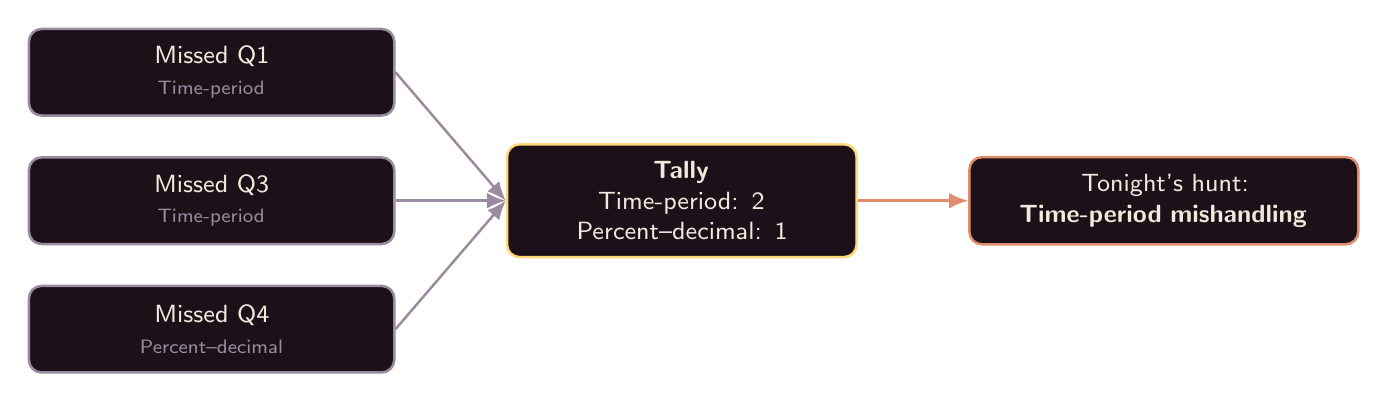
\begin{tikzpicture}[node distance=5mm and 14mm]
  \node[box, text width=42mm] (q1) {Missed Q1\\{\scriptsize\color{Muted}Time-period}};
  \node[box, below=of q1, text width=42mm] (q2) {Missed Q3\\{\scriptsize\color{Muted}Time-period}};
  \node[box, below=of q2, text width=42mm] (q3) {Missed Q4\\{\scriptsize\color{Muted}Percent--decimal}};
  \node[gld, right=of q2, text width=40mm] (tally) {\textbf{Tally}\\Time-period: 2\\Percent--decimal: 1};
  \node[hot, right=of tally, text width=45mm] (first) {Tonight's hunt:\\\textbf{Time-period mishandling}};
  \draw[arrow] (q1.east)--(tally.west);
  \draw[arrow] (q2.east)--(tally.west);
  \draw[arrow] (q3.east)--(tally.west);
  \draw[arrowhot] (tally)--(first);
\end{tikzpicture}
\end{adjustbox}
\end{center}

Nothing in that diagram is a judgement call. The labels come from the vault,
the counting is arithmetic, and the biggest number wins. \themodel\ has not
been asked anything yet.

% =====================================================================
\section{How you beat a snare}

One lucky answer proves nothing, so one lucky answer is not the bar. The loop
runs like this, and it keeps running until you clear the bar or a cap stops it.

\vspace{0.5em}
\begin{center}
\begin{adjustbox}{max width=\textwidth}
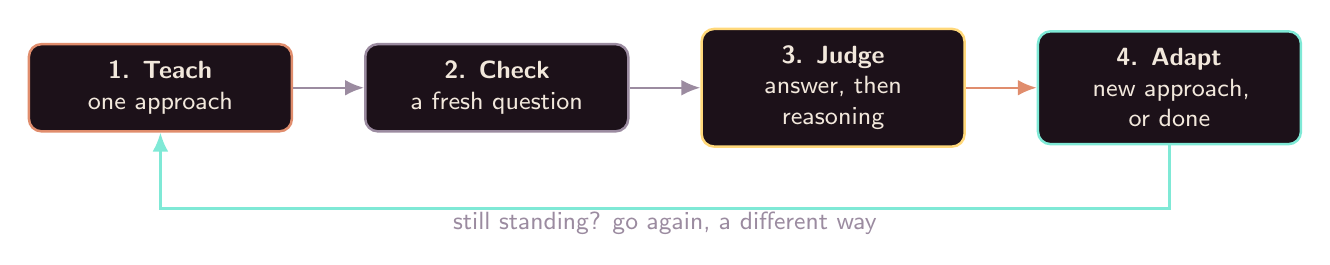
\begin{tikzpicture}[node distance=9mm]
  \node[hot] (teach) {\textbf{1. Teach}\\one approach};
  \node[box, right=of teach] (check) {\textbf{2. Check}\\a fresh question};
  \node[gld, right=of check] (judge) {\textbf{3. Judge}\\answer, then reasoning};
  \node[cool, right=of judge] (adapt) {\textbf{4. Adapt}\\new approach, or done};
  \draw[arrow] (teach)--(check);
  \draw[arrow] (check)--(judge);
  \draw[arrowhot] (judge)--(adapt);
  \draw[arrowcool] (adapt.south) -- ++(0,-8mm) -| (teach.south)
    node[tag, pos=0.25, below] {still standing? go again, a different way};
\end{tikzpicture}
\end{adjustbox}
\end{center}

\subsection{Four ways to explain, and no fifth}

If one explanation does not land, the game does not repeat it louder. It
changes the approach. There are exactly four, fixed in the code, and they are
tried in this order unless \themodel\ argues for a different one.

\vspace{0.3em}
\begin{center}
\begin{tabularx}{0.97\textwidth}{@{}>{\sffamily\bfseries}L{34mm} X@{}}
\toprule
\textcolor{Coral}{Direct correction} & Name the snare plainly --- ``you might think\ldots\ but
actually\ldots'' --- state the right rule in two or three sentences, then work
one example all the way through.\\
\addlinespace[0.3em]
\textcolor{Coral}{Visual walkthrough} & A concrete model walked through one step at a time: a
number line, an area model, groups of objects, a table. The point is to make you
see why it works, instead of handing you another rule to remember.\\
\addlinespace[0.3em]
\textcolor{Coral}{Side-by-side contrast} & The wrong method and the right method on the same
problem, line against line, with a finger on the exact step where they split.\\
\addlinespace[0.3em]
\textcolor{Coral}{Real-world analogy} & Money, pizza slices, game scores. Build the everyday
version first, then map it back onto the maths.\\
\bottomrule
\end{tabularx}
\end{center}

\vspace{0.3em}
When you get a check question wrong, \themodel\ reads what you typed and picks
which of the \emph{remaining} approaches to try next, and says why in one
sentence you can see. It cannot invent a fifth approach, cannot repeat one it
has already used, and cannot leave the ladder. If its answer does not name a
real approach, the code just takes the next rung and says so.

\subsection{The bar, and the three ways a night ends}

\begin{center}
\begin{adjustbox}{max width=\textwidth}
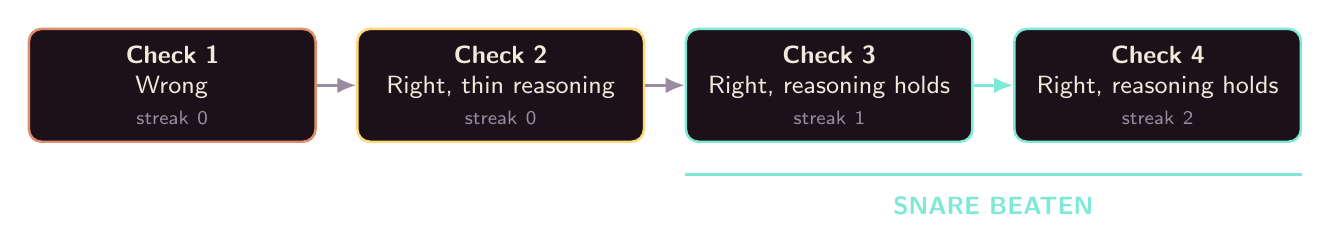
\begin{tikzpicture}[node distance=5mm]
  \node[hot, text width=32mm] (a) {\textbf{Check 1}\\Wrong\\{\scriptsize\color{Muted}streak 0}};
  \node[gld, right=of a, text width=32mm] (b) {\textbf{Check 2}\\Right, thin reasoning\\{\scriptsize\color{Muted}streak 0}};
  \node[cool, right=of b, text width=32mm] (c) {\textbf{Check 3}\\Right, reasoning holds\\{\scriptsize\color{Muted}streak 1}};
  \node[cool, right=of c, text width=32mm] (d) {\textbf{Check 4}\\Right, reasoning holds\\{\scriptsize\color{Muted}streak 2}};
  \draw[arrow] (a)--(b); \draw[arrow] (b)--(c); \draw[arrowcool] (c)--(d);
  \draw[line width=1.2pt, Teal] ([yshift=-4mm]c.south west)--([yshift=-4mm]d.south east)
    node[midway, below=1.5mm, font=\sffamily\small\bfseries, text=Teal]{SNARE BEATEN};
\end{tikzpicture}
\end{adjustbox}
\end{center}

\vspace{0.2em}
The bar is \textbf{two fresh questions right in a row}, with reasoning that
holds up. The reasoning box under each answer is optional and the submit button
never waits on it --- but when you do write something, it counts:

\begin{itemize}
  \item Right answer, reasoning that shows you understand: the streak goes up.
  \item Right answer, thin or circular reasoning: the streak stays where it is.
        You are not punished, but you have not shown anything yet.
  \item Right answer, reasoning that still contains the snare: the streak goes
        back to zero. You got there for the old wrong reason.
  \item Wrong answer: streak to zero, and a different approach next.
\end{itemize}

Three caps end the night, and all three are plain code: \textbf{four} check
questions, \textbf{twelve} model calls, or a ladder with no rungs left. When
one of them trips, the game stops and says which one. It does not drill you
into the ground, and it does not pretend.

\begin{quietbox}
\textbf{A fresh question is fresh, but it is not random.} Every follow-up is
modelled on the exact question you just got wrong, and stays on that same
topic. Not merely the same part of the course --- slope from two points and the
distributive property are both Algebra, and a player who could not solve the
equation is not helped by coordinate geometry. If the vault has nothing left on
that exact topic, the game would rather write a new question than hand you the
wrong one.
\end{quietbox}

% =====================================================================
\section{What the vault holds}

\begin{itemize}
  \item \textbf{55 questions} across the five parts of the course: Number,
        Algebra, Financial Literacy, Geometry \& Measurement, Data. The bank
        was audited against the published Grade 9 expectations and against what the
        EQAO assessment actually covers.
  \item \textbf{A worked solution on every single one.} That is what lets
        \themodel\ teach without being allowed to calculate.
  \item \textbf{A snare on every wrong option} --- 165 of them --- naming the
        faulty thinking that produces exactly that answer.
  \item \textbf{A balanced key}, 14/14/14/13 across A, B, C and D.
  \item \textbf{A topic on every question}, and the topic is a hard filter when
        the game hunts for your next one, not a preference.
\end{itemize}

Finding a follow-up is a tag lookup, not a search: the vault knows that NUM-6
and NUM-6b are the same idea at two depths, and it will take a sibling before
it takes a stranger. If nothing on your topic is left, it returns nothing ---
and returning nothing is a real answer. The game then writes a question under
audit, or stops and says the vault is out. Either beats practising the wrong
thing.

% =====================================================================
\section{Ten jobs for \themodel, one door}

\themodel\ is not decoration on top of a quiz app. Take it out and there is no
lesson, no judgement, no direction, and no letter home --- just a marked test.
Here is every job it does.

\vspace{0.3em}
\begin{center}\small
\begin{tabularx}{\textwidth}{@{}>{\sffamily\bfseries\color{Gold}}c >{\sffamily\bfseries}L{53mm} X@{}}
\toprule
& \textcolor{Gold}{\sffamily THE JOB} & \textcolor{Gold}{\sffamily WHAT CODE STILL OWNS}\\
\midrule
1 & Writes the lesson & The approach, and the verified working it may not contradict\\
\addlinespace[0.2em]
2 & Explains why your wrong answer felt right & The right answer; it may not redo the arithmetic\\
\addlinespace[0.2em]
3 & Gives a hint without giving it away & How deep the hint may go\\
\addlinespace[0.2em]
4 & Judges whether your reasoning holds up & Three labels and no fourth; whether the answer was right\\
\addlinespace[0.2em]
5 & Chooses the next approach, and says why & The four approaches, and the order if the reply is unusable\\
\addlinespace[0.2em]
6 & Writes a fresh question when the vault is out & The topic, and a refusal if the question drifts off it\\
\addlinespace[0.2em]
7 & Solves that question again, blind & Whether the two answers match, and what happens if not\\
\addlinespace[0.2em]
8 & Decides which fight comes next & The list it may choose from: real fights, still open\\
\addlinespace[0.2em]
9 & Speaks as the citadel --- taunts, reactions, relics & That none of it touches your score\\
\addlinespace[0.2em]
10 & Writes the note that goes home & Every single figure on that page\\
\bottomrule
\end{tabularx}
\end{center}

\vspace{0.5em}
Read that table as one evening rather than a list. You miss a question, so it
explains why your answer felt right (2). It teaches the idea properly (1). The
vault has nothing left on your topic, so it writes you a fresh one (6) and then
solves that question again, blind, to check its own key (7). You answer and you
type why --- and it decides whether that reasoning actually holds (4). It does
not, quite, so it picks a different way to explain and tells you which and why
(5). Then the night ends and it writes home (10).

Two of those jobs turn up twice over. Number one also works down at the
Collector's training ground, where \themodel\ whispers the mental shortcut
before you go in; number four works there too, reading the exact questions you
missed afterwards and naming the one pattern in them. Same door, same caps,
different room.

\begin{quietbox}
\textbf{One door, and what it buys.} Every prompt and every reply in this game
passes through a single function. That is why the caps can be counted at all.
It is why the whole app moves to a bigger or a smaller \themodel\ by changing
one environment variable, with nothing else to edit. And it is why a model that
is slow, busy, or simply not installed makes the game go quiet rather than
crash --- the door hands back clearly marked placeholder text, and the battle,
the marking and the vault carry on without it.
\end{quietbox}

% =====================================================================
\section{True and judged}

Here is the line the whole design is built on. Code owns what is \textbf{true}.
\themodel\ owns what is \textbf{judged}. Nothing crosses.

\vspace{0.5em}
\begin{center}
\begin{adjustbox}{max width=\textwidth}
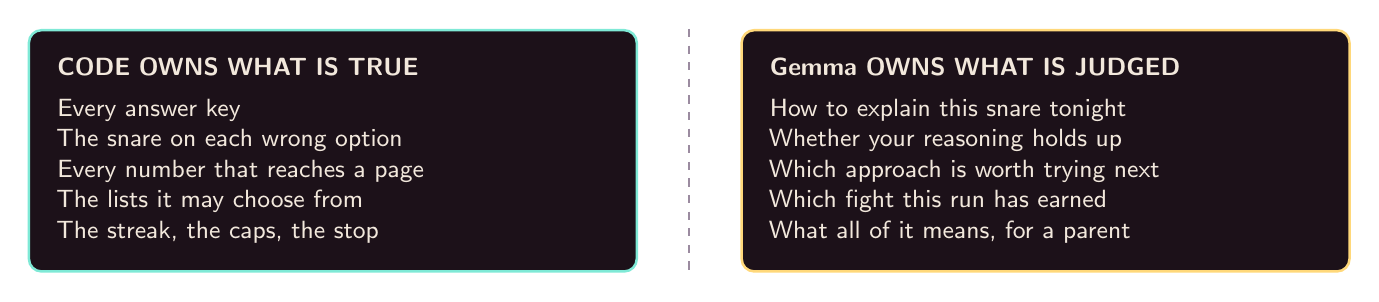
\begin{tikzpicture}
  \node[cool, text width=70mm, align=left, minimum height=0mm, inner sep=3.6mm] (L)
    {\textbf{CODE OWNS WHAT IS TRUE}\\[0.4em]
     Every answer key\\
     The snare on each wrong option\\
     Every number that reaches a page\\
     The lists it may choose from\\
     The streak, the caps, the stop};
  \node[gld, text width=70mm, align=left, minimum height=0mm, inner sep=3.6mm,
        right=13mm of L] (R)
    {\textbf{\themodel\ OWNS WHAT IS JUDGED}\\[0.4em]
     How to explain this snare tonight\\
     Whether your reasoning holds up\\
     Which approach is worth trying next\\
     Which fight this run has earned\\
     What all of it means, for a parent};
  \draw[Muted, line width=0.9pt, dashed]
    ($(L.north east)!0.5!(R.north west)$) -- ($(L.south east)!0.5!(R.south west)$);
\end{tikzpicture}
\end{adjustbox}
\end{center}

\vspace{0.2em}
Every one of those left-hand rows is there because we watched the right-hand
side get something wrong first. Four shields came out of that.

\begin{shieldbox}
\textbf{Shield 1 --- \themodel\ never redoes the maths.}\\
Asked to re-explain a question it had already solved, it would quietly redo the
sums and land somewhere new, in confident prose, right next to the correct
answer. So the verified working now rides inside the prompt as the only
arithmetic it is allowed to state. Its job is to explain \emph{why} your method
fails, never to recompute.
\end{shieldbox}

\begin{shieldbox}
\textbf{Shield 2 --- the snare is read, not guessed.}\\
Every wrong option in the vault carries the faulty thinking that produces it.
When you pick one, the game looks the snare up. No model call, no inference, no
chance of naming the wrong trap and teaching you a lesson you did not need.
\end{shieldbox}

\begin{shieldbox}
\textbf{Shield 3 --- a written question must survive itself.}\\
We caught the model writing a perfectly good question and marking the wrong
option as the answer. A student would have been told they were wrong for being
right. So now anything \themodel\ writes has to solve itself again \emph{blind}
--- without seeing the key it just wrote --- and the two answers have to match.
They disagree, the question is destroyed and nobody ever sees it.
\end{shieldbox}

\vspace{0.4em}
\begin{center}
\begin{adjustbox}{max width=\textwidth}
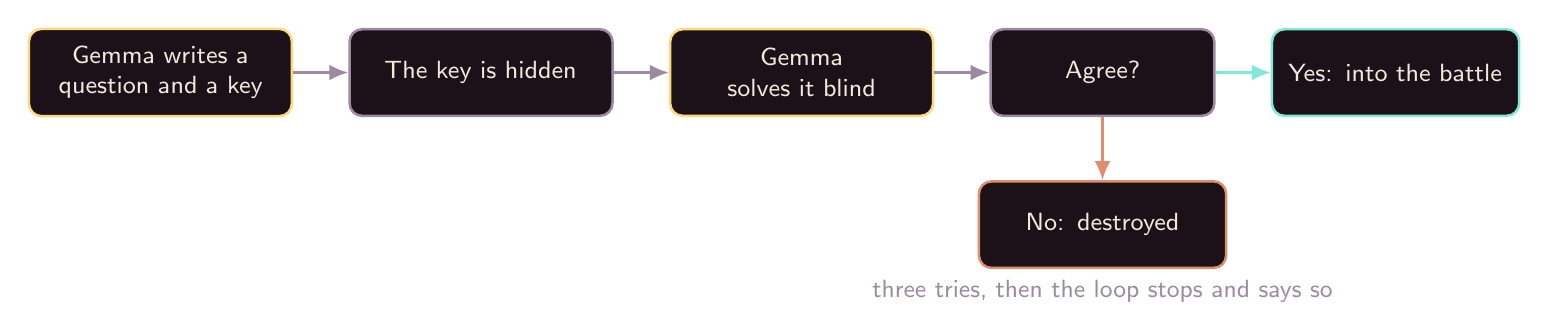
\begin{tikzpicture}[node distance=7mm]
  \node[gld] (write) {\themodel\ writes a question and a key};
  \node[box, right=of write] (hide) {The key is hidden};
  \node[gld, right=of hide] (solve) {\themodel\ solves it blind};
  \node[box, right=of solve, text width=24mm] (match) {Agree?};
  \node[cool, right=of match, text width=27mm] (show) {Yes: into the battle};
  \node[hot, below=8mm of match, text width=27mm] (bin) {No: destroyed};
  \draw[arrow] (write)--(hide);
  \draw[arrow] (hide)--(solve);
  \draw[arrow] (solve)--(match);
  \draw[arrowcool] (match)--(show);
  \draw[arrowhot] (match)--(bin);
  \node[tag, below=1mm of bin] {three tries, then the loop stops and says so};
\end{tikzpicture}
\end{adjustbox}
\end{center}

\begin{shieldbox}
\textbf{Shield 4 --- \themodel\ may not put a number on the page.}\\
It once wrote ``beaten three tricks'' when one had been beaten, borrowing a 3
that belonged to a different count on the same screen. Checking figures one at
a time cannot catch a real number attached to the wrong noun. So the rule is
absolute: on the page that goes to a parent, code prints every figure and
\themodel\ prints none. Any reply containing a number --- in digits or spelled
out --- is thrown away and a sentence built from the same facts goes out
instead.
\end{shieldbox}

\vspace{0.3em}
There is a fifth guard that is not about the model at all. In an early draft of
the vault, 58\% of the correct answers sat on option A. A player who always
guessed A would have scored well and learnt nothing. The key is now balanced
across all four letters, and every note about a wrong answer is keyed to the
answer's \emph{text}, so it stays true however the options are shuffled.

\begin{quietbox}
Underneath all of it, one sentence: \textbf{a small model is a capable judge and
an unreliable authority.} Everything \themodel\ says in this game is a
judgement. Nothing it says is the source of what is mathematically true.
\end{quietbox}

% =====================================================================
\section{When the snare holds}

Some nights you do not beat it. The game does not keep grinding. It says the
battle is ending, why it is ending, and that a person is probably more use than
another question right now. A note goes home naming the approaches already
tried, so nobody starts from scratch.

That is also when the Collector notices you. He is the giant skull above the
citadel, and the five monsters are afraid of him. He does not test new ideas.
He tests the arithmetic you are supposed to already own, and he tests it
against a clock: \textbf{ten questions, eight seconds each, three lives}.
Nothing in his arena counts against your quiz record.

Lose to him and you go down to his lieutenants, one mental shortcut each.

\vspace{0.4em}
\begin{center}
\begin{tabularx}{0.97\textwidth}{@{}>{\sffamily\bfseries\color{Coral}}l X@{}}
\toprule
Twinfang & Doubling and halving. Double by adding a number to itself; multiply
by 4 by doubling twice.\\
\addlinespace[0.25em]
The Niner & Nines, fast. Multiply by 10, then subtract the number once.\\
\addlinespace[0.25em]
Splitjaw & Making tens. $47+38$ becomes $47+3$, then $+35$.\\
\bottomrule
\end{tabularx}
\end{center}
\vspace{0.4em}

Each drill is ninety seconds on three lives. \themodel\ whispers the shortcut
before you go in, reads the exact questions you missed afterwards, and picks
the one trick worth drilling next. Then it chooses which lieutenant is worth
your time --- from the list of the ones you have actually fought, with the
scores you actually got, and it names that evidence out loud when it sends you.

Retreating from any fight is free. The monsters remember it, and they will
mention it when you come back.

% =====================================================================
\section{A letter reaches home}

After a battle, a note is written for whoever is at home. Not only on the bad
nights --- a parent who only hears from us on the worst day cannot see a
pattern, so notes go after any battle with mistakes in it, after a hand-off,
and after a win.

The note says which monster was fought, which snare caught you most, which
explanations were tried, whether the snare fell or is still standing, and three
things to try at the kitchen table with coins, cups, food or paper. Ten
minutes, no jargon, nothing to buy. And it is about one evening --- it is not a
label anyone gets to keep.

One button on that page prints a practice sheet: up to ten questions on that
one snare, room to write under each, and the answer key on its own page so a
parent can hand over the questions without handing over the answers. Vault
questions first, because those come with working a parent can check. Anything
\themodel\ writes to fill the sheet has already solved itself blind, the same as
on screen. If it cannot fill ten, the sheet comes out short. It never comes out
with a question we could not verify.

% =====================================================================
\section{It really runs, and it runs on one laptop}

\begin{center}
\begin{adjustbox}{max width=\textwidth}
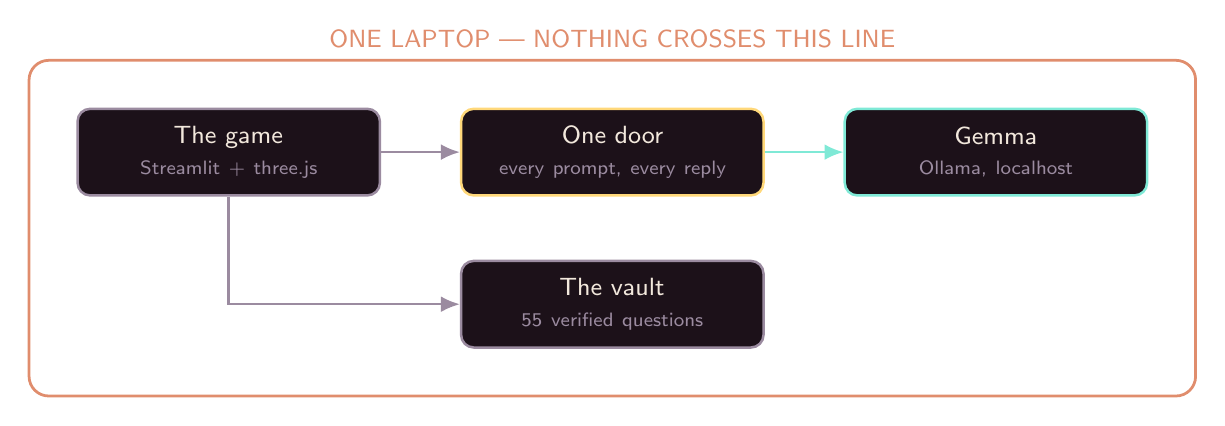
\begin{tikzpicture}[node distance=6mm]
  \node[box, text width=34mm] (ui) {The game\\{\scriptsize\color{Muted}Streamlit + three.js}};
  \node[gld, right=10mm of ui, text width=34mm] (door) {One door\\{\scriptsize\color{Muted}every prompt, every reply}};
  \node[cool, right=10mm of door, text width=34mm] (model) {\themodel\\{\scriptsize\color{Muted}Ollama, localhost}};
  \node[box, below=8mm of door, text width=34mm] (vault) {The vault\\{\scriptsize\color{Muted}55 verified questions}};
  \draw[arrow] (ui)--(door);
  \draw[arrowcool] (door)--(model);
  \draw[arrow] (ui.south) |- (vault.west);
  \node[draw=Coral, line width=1pt, rounded corners=2.5mm,
        fit=(ui)(door)(model)(vault), inner sep=6mm] (laptop) {};
  \node[tag, text=Coral, above=1mm of laptop.north] {ONE LAPTOP --- NOTHING CROSSES THIS LINE};
\end{tikzpicture}
\end{adjustbox}
\end{center}

\vspace{0.3em}
The whole game exists and you can play it end to end today: the opening scene,
the citadel you can orbit, five monster halls, the training loop, the Collector
and his three lieutenants, the notes home and the printable sheets, and the
gate that opens when the last seal breaks.

No account. No sign-in. No internet needed once it is installed. Three.js is
vendored into the repository, the monster models are CC0, the audio is ours,
and there is not a single request to a CDN. A fourteen-year-old's worked-out
mistakes are exactly the kind of thing that should not be uploaded anywhere, so
they are not. They stay in a file on the family's own machine.

And if \themodel\ is not installed at all, the app still opens, still runs the
quiz, still marks it, and says plainly where the writing would have been.

% =====================================================================
\vfill
{\color{Muted}\hrule height 0.4pt}
\vspace{0.6em}
\begin{center}
{\sffamily\small\bfseries\color{Coral}Gokulakrishnan $\cdot$ Padmanabha $\cdot$
Taha $\cdot$ Naimah $\cdot$ Amarah}\\[0.3em]
{\small\color{Muted}Build with AI --- \themodel\ Hackathon $\cdot$ GDG Windsor
$\cdot$ Edge / On-Device}
\end{center}

\end{document}
